\chapter{LITERATURE REVIEW}

Generalized eigenvalue problems involving symmetric and positive definite matrices are fundamental in numerical linear algebra with applications in structural  dynamics, quantum mechanics, and control theory. Solving these kind of problems involve computing the eigenvalues $\lambda$ and eigenvectors $v$ that satisfies the equation. The choice of method depends on the properties of the matrix involved in the problem we are trying to solve (e.g, sparsity, symmetry) and computational constraints. In this chapter, we discuss some of the research that has been done on this topic.\par
Golb \& Van Loan, $2013$ considered the case when B is invertible, in which the problem is reduced to $B^{-1}Av = \lambda v$. However, explicity forming $B^{-1}A$ is numerically unstable if B is ill-conditioned. Since $B$ a symmetric and positive definite $B$, one can compute a Cholesky factorization $B = LL^{T}$ which allows us to  reduce the equation to a standard eigenvalue problem $L^{-1}AL^{-T}y = \lambda y$ where $y= L^T v$, which can then be solved by using the symmetric $QR$ algorithm to compute a Schur decomposition.\par
The $QZ$ algorithm (Moler and Stewart, 1973) for the non-symmetric GEP, is an iterative method that generalized the $QR$ algorithm, to handle singular or ill-conditioned $B$. It applies orthogonal transformations to simutaneously reduce $A$ and $B$ to upper triangular forms from which the eigenvalues are extracted. Although this method is robust and backward stable, it is computationally expensive, thereby limiting its use to small or medium sized matrices.\par

And as an example of citing things, I'm going to cite a brilliant paper - \citep{jones_2016}. See bibliography.bib for doing references.

\begin{figure*}
	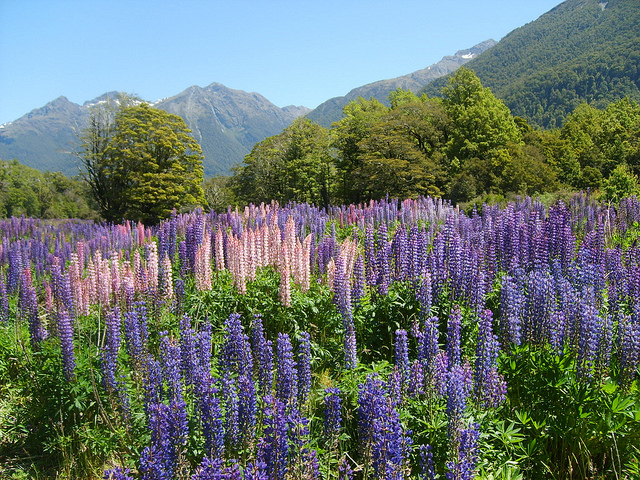
\includegraphics[height =5in]{./Plots/nature.jpg}
	\caption{An individual figure!}
\end{figure*}
        
\begin{figure*}[h]
	\subfloat[\label{fig:HD8538_ellplot}]{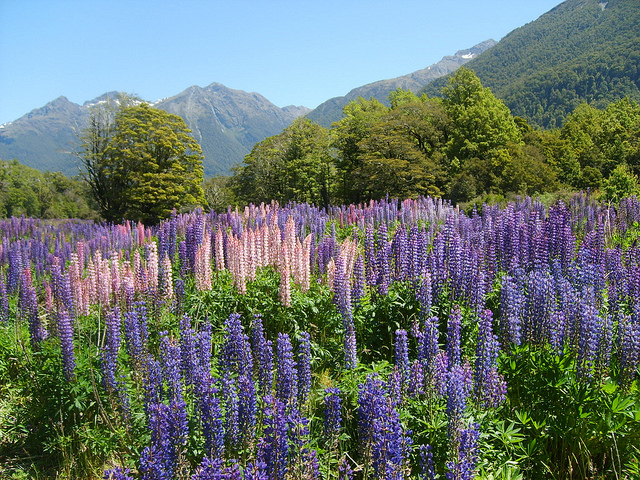
\includegraphics[height =2.5in]{./Plots/nature.jpg}} 
	\subfloat[\label{fig:HD8538_phot}]{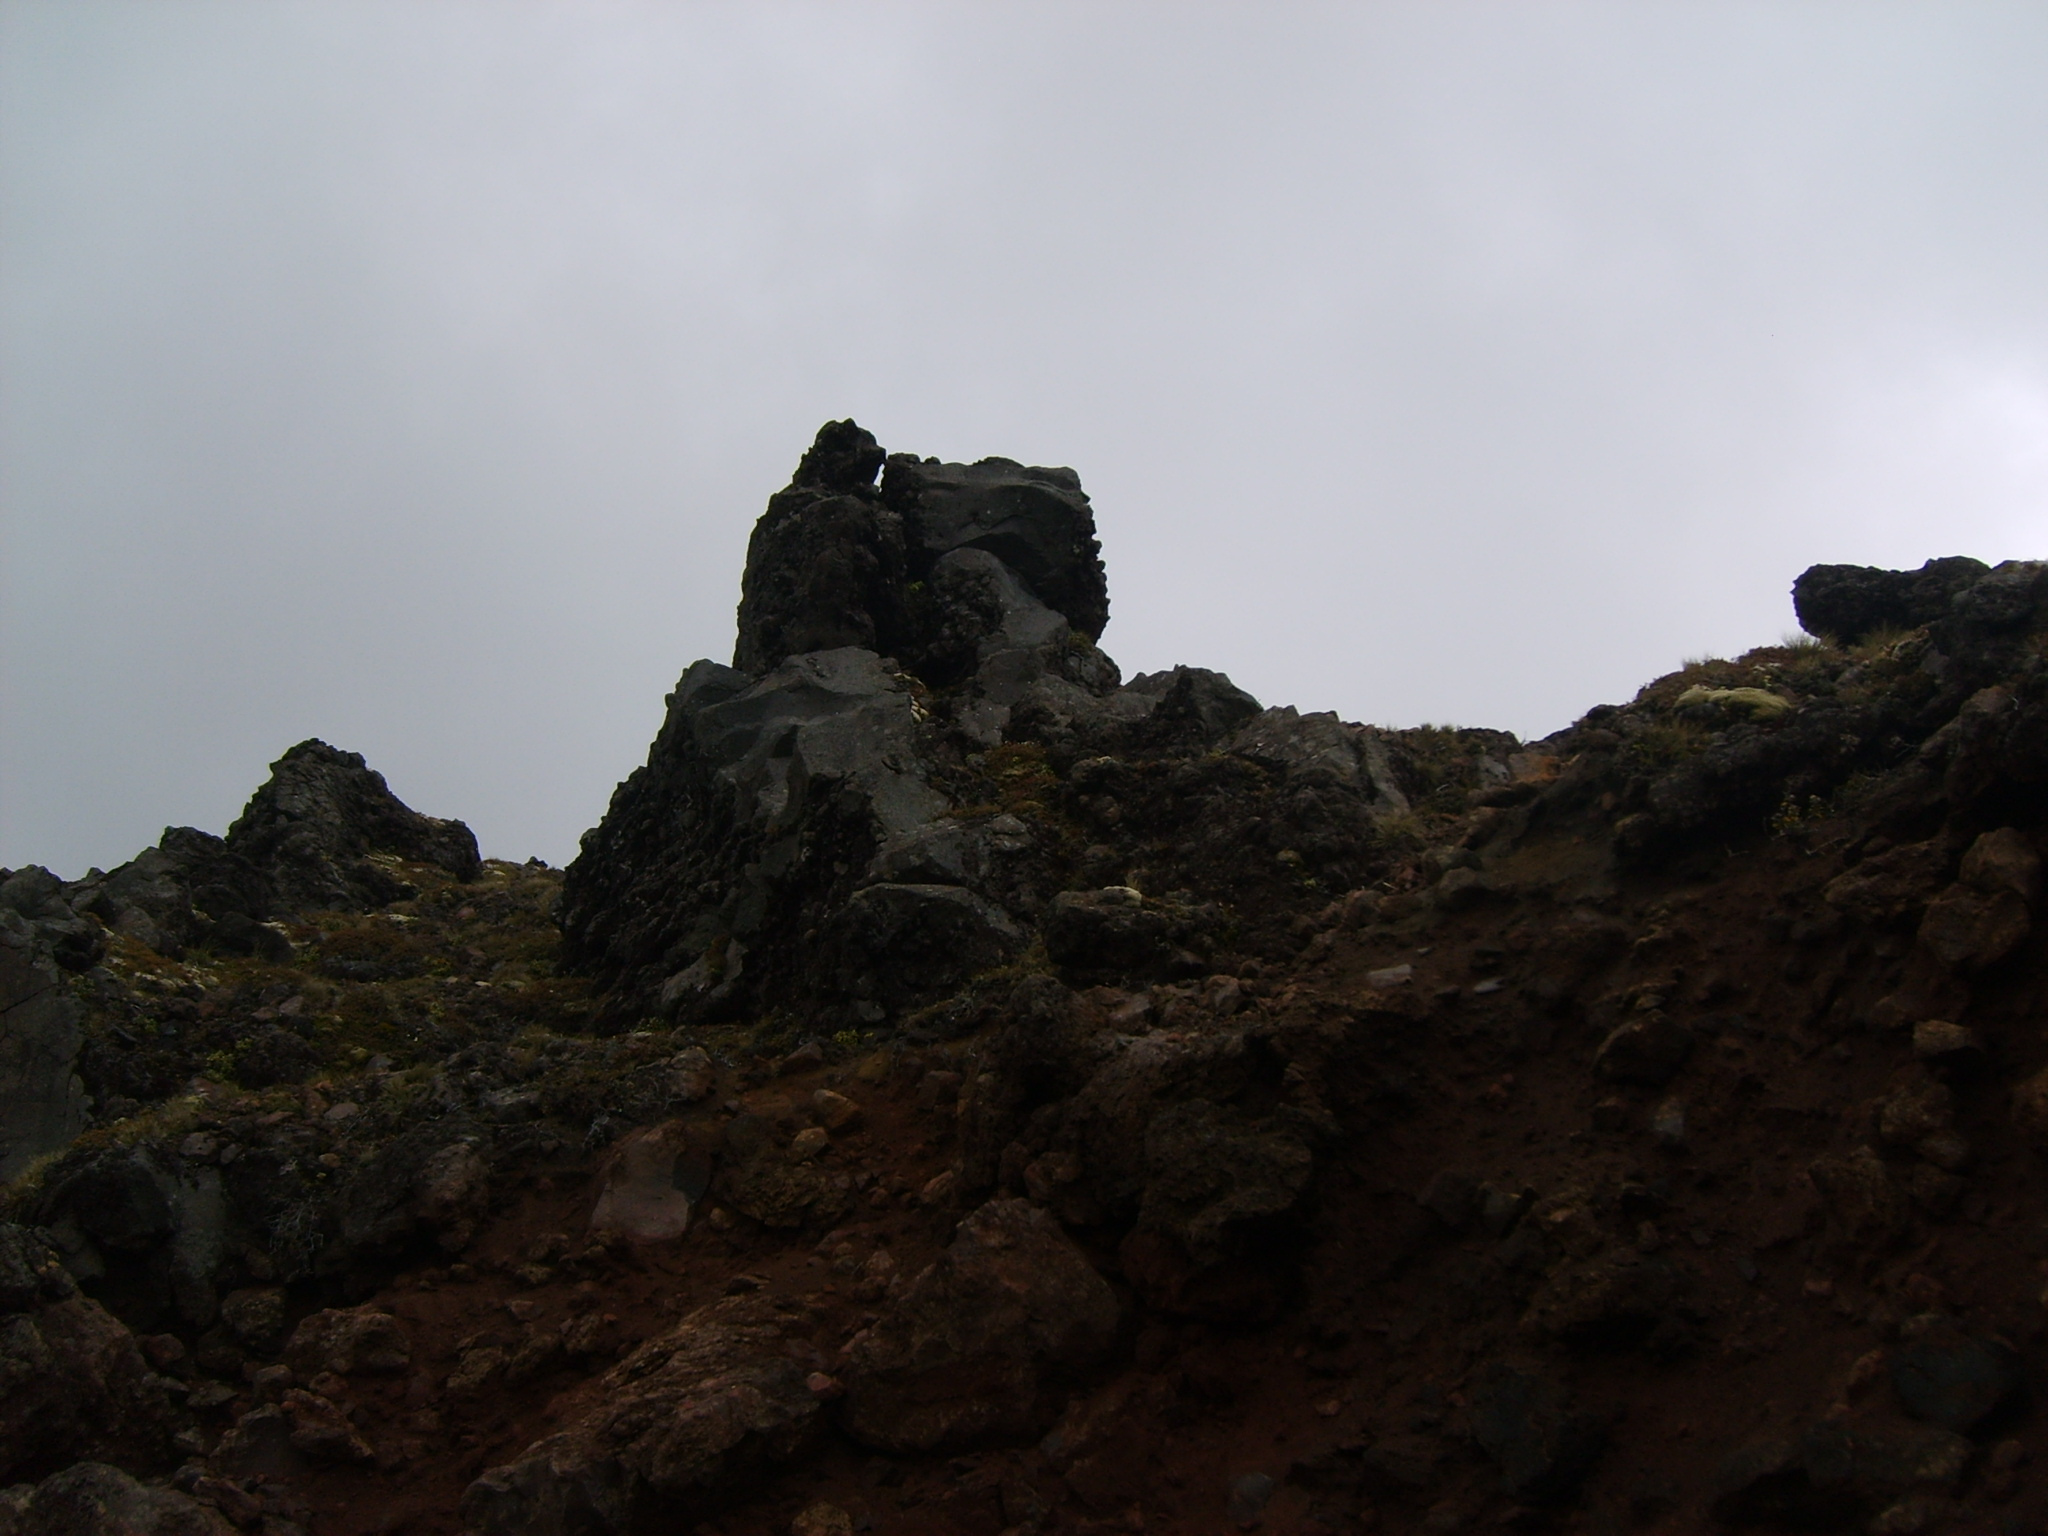
\includegraphics[height =2.5in]{./Plots/rocks.jpg}} \\
	\subfloat[\label{fig:HD8538_vis}]{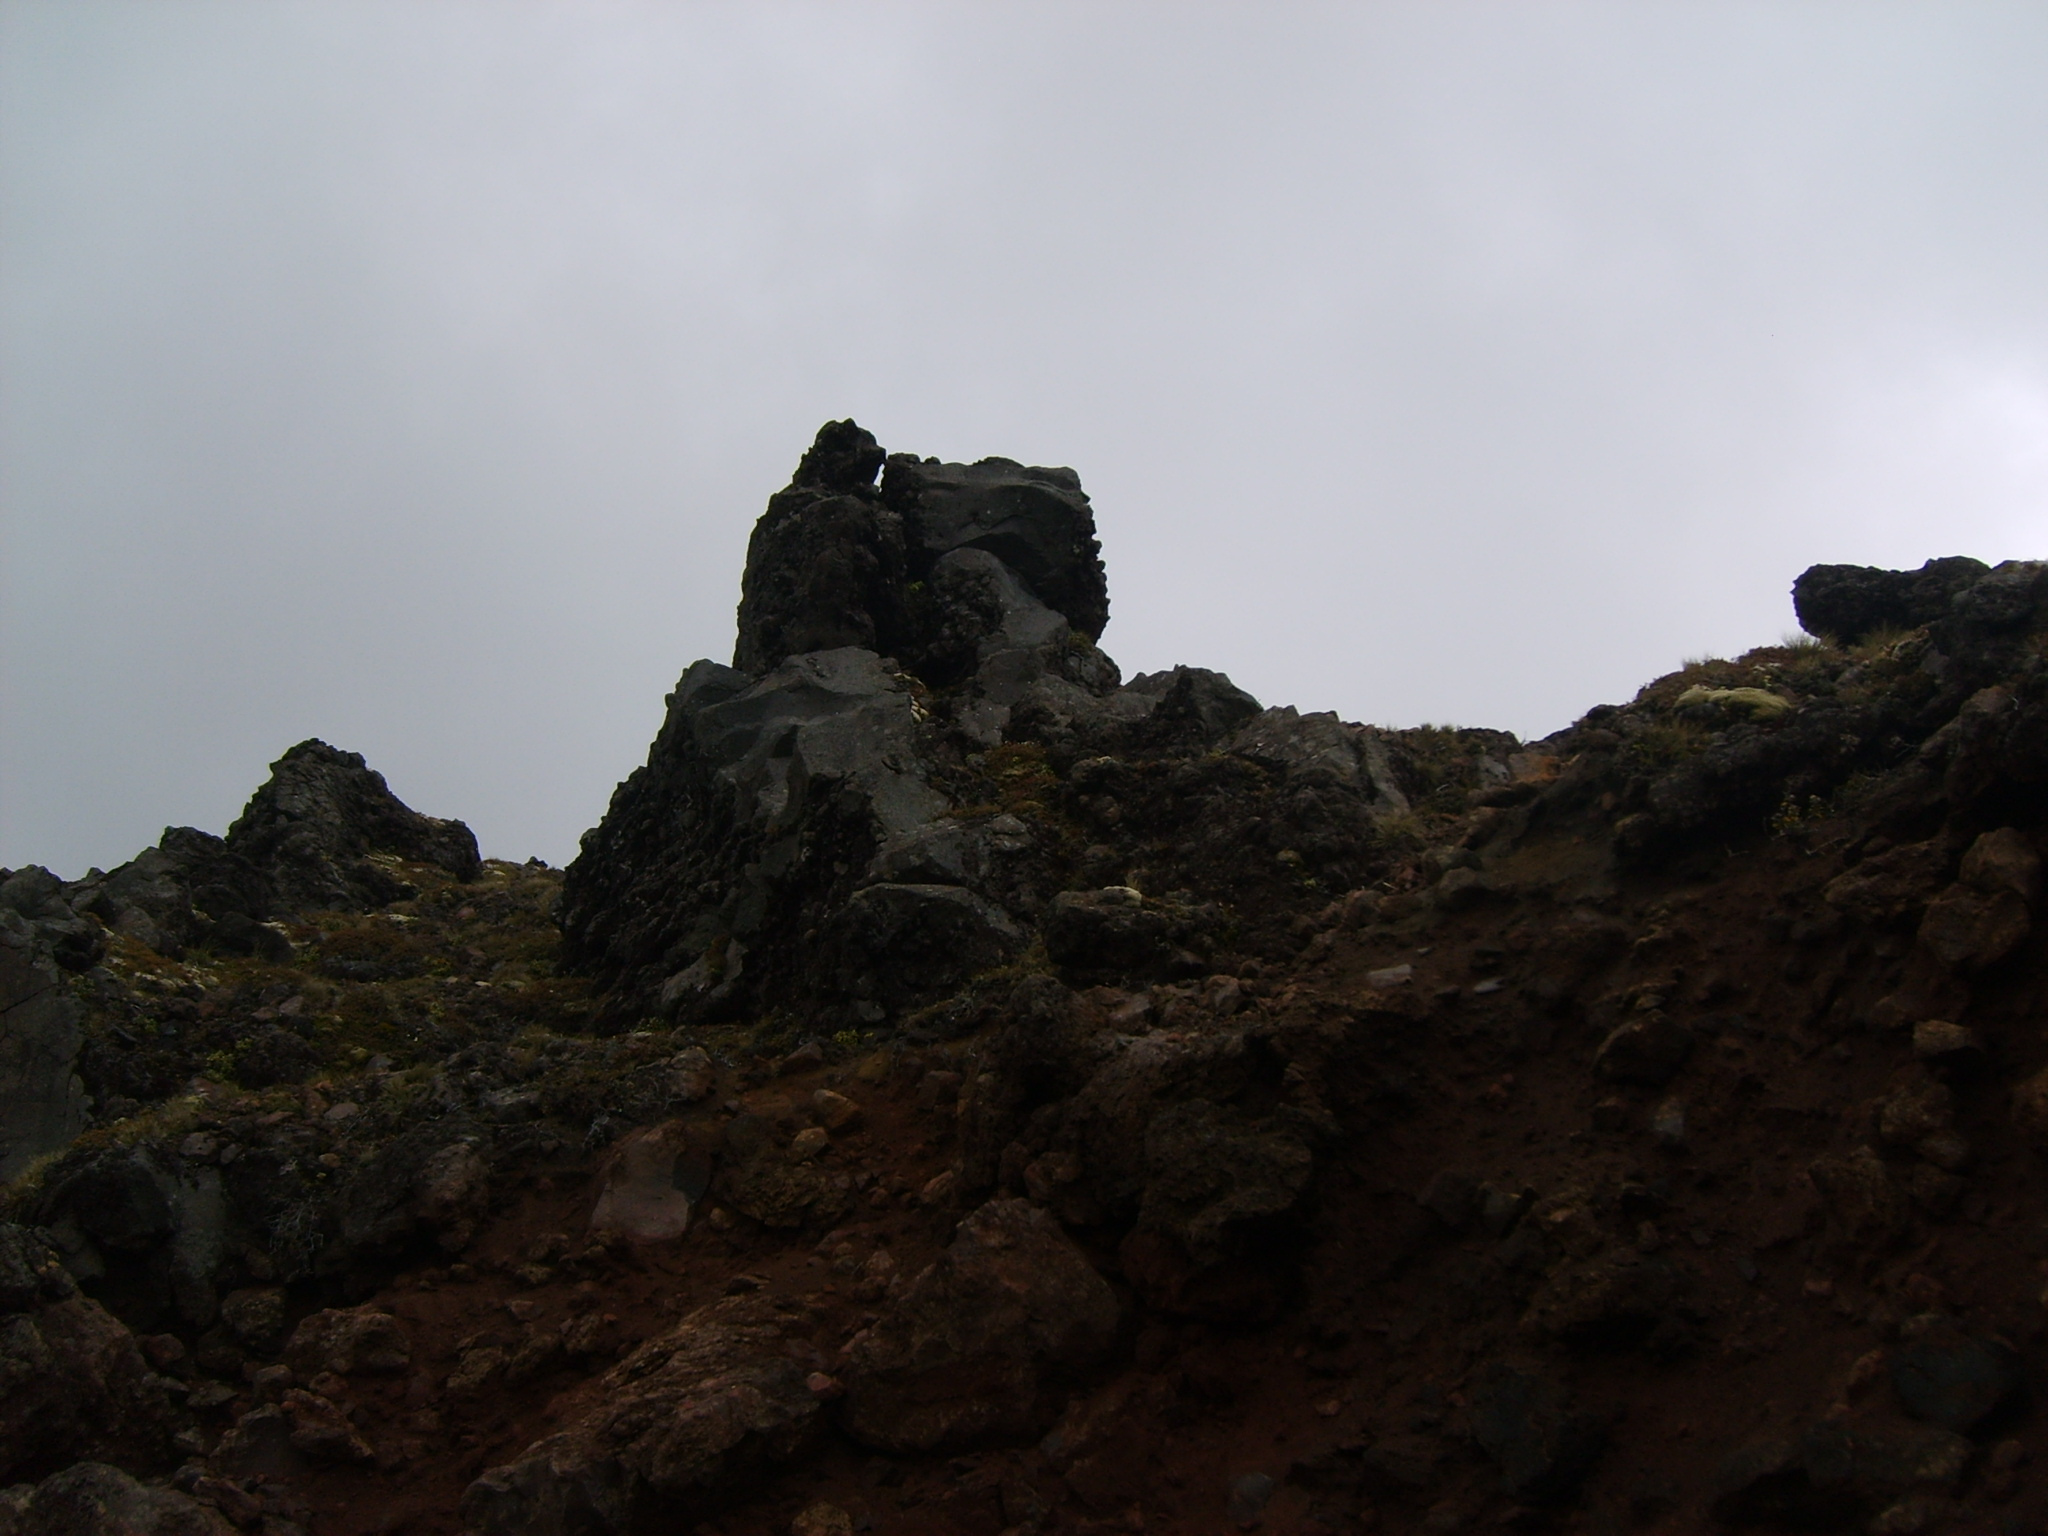
\includegraphics[height =2.5in]{./Plots/rocks.jpg}}
	\subfloat[\label{fig:HD8538_HRD}]{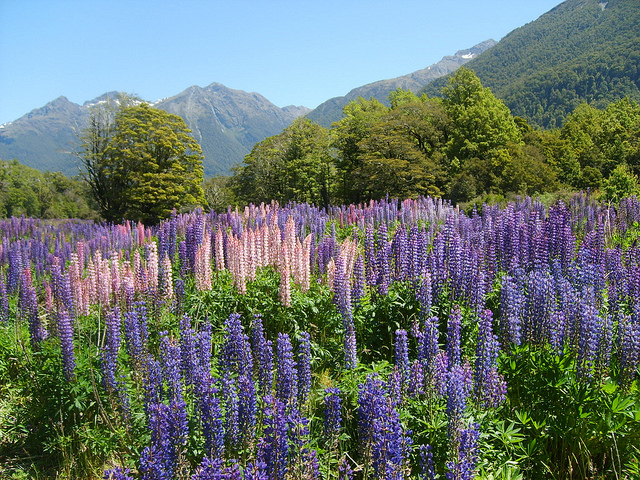
\includegraphics[height =2.5in]{./Plots/nature.jpg}}
	\caption{Multiple figures!}
\end{figure*}



\begin{landscape}
\begin{longtable}{cccccccccccccc}
\label{tab:disk}\\
\caption{Insert Table Caption here}\\
\hline\endhead  % header material
\hline\endfoot  % footer material
\hline
Blah & Blah & Blah \\
\hline
Stuff & Things & etc. \\
\nodata & \nodata & \nodata \\
\end{longtable}
\end{landscape}
